\documentclass[12pt,fleqn,handout]{beamer}


\xdefinecolor{lavendar}{rgb}{0.8,0.6,1}
\xdefinecolor{olive}{cmyk}{0.64,0,0.95,0.4}
%\xdefinecolor{olive}{cmyk}{1,0,0,0}
\xdefinecolor{mag}{cmyk}{0.1,1,0,0.2}
\xdefinecolor{lblue}{rgb}{0,0,1.5}
\xdefinecolor{lred}{rgb}{1,0,0}
\xdefinecolor{mine}{cmyk}{1,0,0.2,0}
\xdefinecolor{bluel}{cmyk}{0.1,0,0.9,0.4}

\usepackage{amsmath,amssymb,dsfont,mathrsfs}
\usepackage{tikz,pgflibraryplotmarks}
\usepackage{multimedia}
\usepackage{wasysym}
\usepackage{rotating}
\usepackage{algorithm,algorithmic}
\usepackage{graphicx} % more modern
\usepackage{subfigure}
\usepackage{booktabs}

\usepackage{pgfplots}
\usepackage{verbatim}

\usepackage{setspace}
\newlength\iwidth
\newlength\iheight

\newcommand\makebeamertitle{\frame{\maketitle}}%
\graphicspath{{./images/}}
\setbeamertemplate{navigation symbols}{}
\addtobeamertemplate{navigation symbols}{}{%
    \usebeamerfont{footline}%
    \usebeamercolor[fg]{footline}%
	\insertshorttitle
    \;--
    \insertframenumber
}

\newcommand{\sectionstart}{
	\only<beamer>{
 	\begin{frame}% (fold)
 		\begin{centering}\Huge \insertsection \par\end{centering}
 	\end{frame}% frame the_application (end)
	}
 }


% make bibliography entries smaller
\usepackage{natbib}
\setbeamertemplate{bibliography item}{[\theenumiv]}
\renewcommand\bibfont{\scriptsize}
\setbeamertemplate{frametitle continuation}[from second]
\newcommand{\tcr}{\textcolor{red}}
\newcommand{\tcrd}{\textcolor{red}}
\newcommand{\tcb}{\textcolor{bluel}}
\newcommand{\tcm}{\textcolor{mag}}
\newcommand{\tcg}{\textcolor{olive}}

\newcommand{\R}{\mathbb{R}}
\newcommand{\C}{\mathbb{C}}

% bold lower-case for vectors
\newcommand{\bfa}{{\bf a}}
\newcommand{\bfb}{{\bf b}}
\newcommand{\bfc}{{\bf c}}
\newcommand{\bfs}{{\bf s}}
\newcommand{\bfm}{{\bf m}}
\newcommand{\bfd}{{\bf d}}
\newcommand{\bfe}{{\bf e}}
\newcommand{\bfu}{{\bf u}}
\newcommand{\bfy}{{\bf y}}
\newcommand{\bfx}{{\bf x}}
\newcommand{\bfh}{{\bf h}}
\newcommand{\bfw}{{\bf w}}
\newcommand{\bfv}{{\bf v}}
\newcommand{\bfr}{{\bf r}}
\newcommand{\bfz}{{\bf z}}
\newcommand{\bfp}{{\bf p}}


% bold upper-case for linear operators
\newcommand{\bfA}{{\bf A}}
\newcommand{\bfB}{{\bf B}}
\newcommand{\bfZ}{{\bf Z}}
\newcommand{\bfM}{{\bf M}}
\newcommand{\bfC}{{\bf C}}
\newcommand{\bfD}{{\bf D}}
\newcommand{\bfQ}{{\bf Q}}
\newcommand{\bfJ}{{\bf J}}
\newcommand{\bfG}{{\bf G}}
\newcommand{\bfI}{{\bf I}}
\newcommand{\bfP}{{\bf P}}
\newcommand{\bfK}{{\bf K}}
\newcommand{\bfY}{{\bf Y}}
\newcommand{\bfW}{{\bf W}}
\newcommand{\bfR}{{\bf R}}
\newcommand{\bfL}{{\bf L}}
\newcommand{\bfF}{{\bf F}}
\newcommand{\bfT}{{\bf T}}
\newcommand{\bfS}{{\bf S}}
\newcommand{\bfX}{{\bf X}}
\newcommand{\bfU}{{\bf U}}
\newcommand{\bfV}{{\bf V}}
\newcommand{\bfH}{{\bf H}}


\newcommand{\calF}{\mathcal{F}}



\newcommand{\hf}{{\frac 12}}
\newcommand{\bftheta}{{\boldsymbol \theta}}
\newcommand{\bfxi}{{\boldsymbol \xi}}

\newcommand{\bfLambda}{{\boldsymbol \Lambda}}
\newcommand{\bfSigma}{{\boldsymbol \Sigma}}
\newcommand{\bfepsilon}{{\boldsymbol \epsilon}}

\newcommand{\E}{\vec E}
\newcommand{\B}{\vec B}

\newcommand{\vu}{  {\vec {\bf u}}}

\newcommand{\grad}{  {\vec {\bf \nabla}}}

\newcommand{\lfrownie}{\textcolor{red}{\large{\frownie}}}
\newcommand{\lsmiley}{\textcolor{green}{\large{\smiley}}}

\newcommand{\curl}{\ensuremath{\nabla\times\,}}
\renewcommand{\div}{\nabla\cdot\,}
\newcommand{\divh}{\nabla_h\cdot\,}
\renewcommand{\grad}{\ensuremath{\nabla}}

\DeclareMathOperator*{\argmin}{arg\,min}


\title{Introduction to Nonlinear Models}
\subtitle{Numerical Methods for Deep Learning}
\date{}

\begin{document}

\makebeamertitle

\begin{frame}\frametitle{Motivation: Nonlinear Models}


In general, impossible to find a linear separator between classes
%$$ \bfC = \bfX \bfW + b $$

\begin{center}
	\begin{tabular}{cc}
		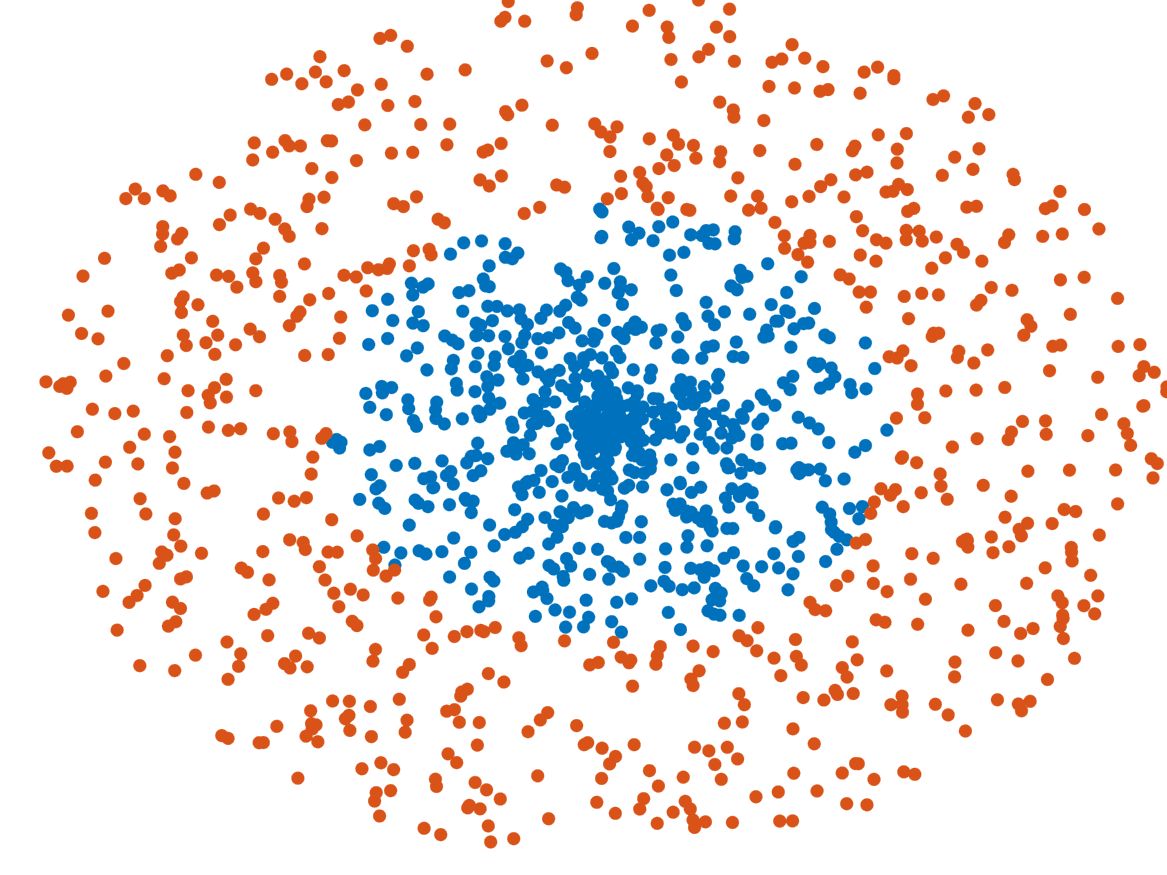
\includegraphics[width=45mm]{Circle-train} & 
		\invisible<beamer|1>{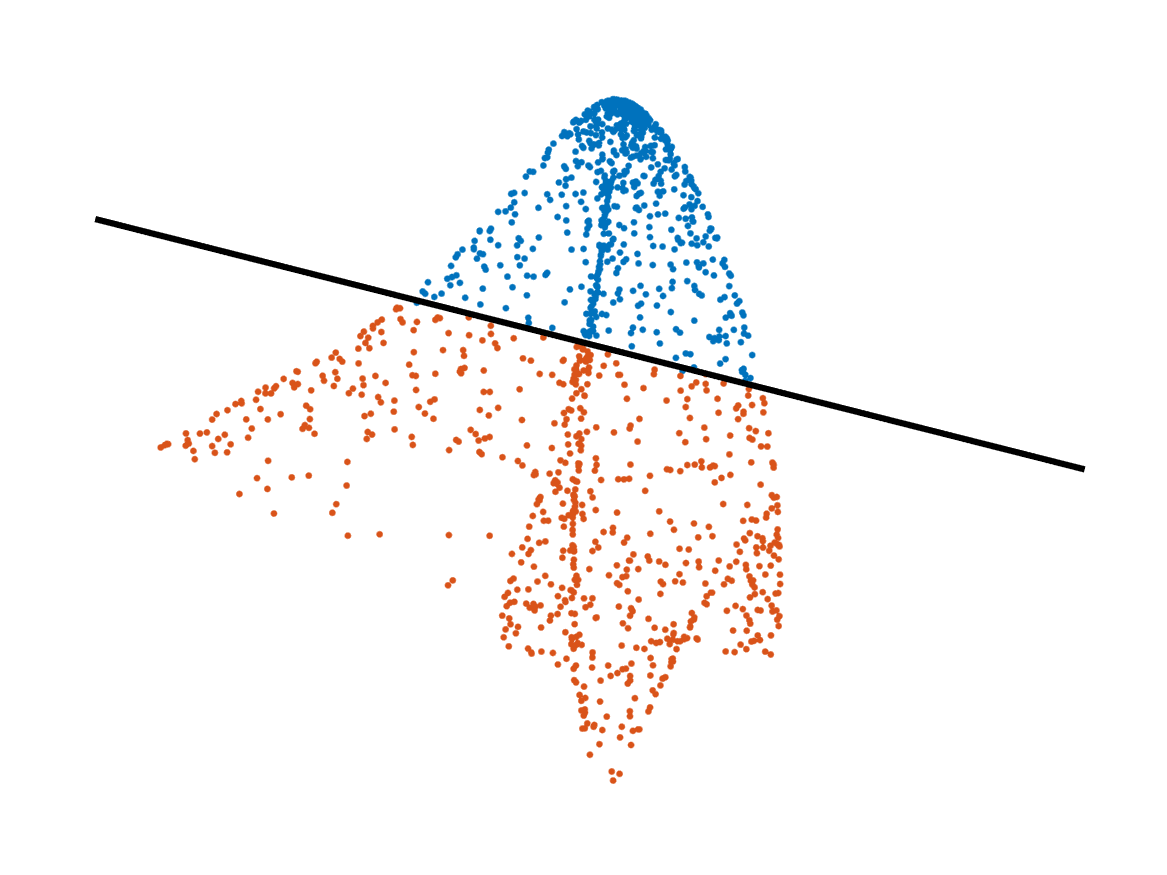
\includegraphics[width=45mm]{Circle-proptrain} }\\
		input features & \invisible<beamer|1>{transformed features}
	\end{tabular}
\end{center}

\bigskip

\invisible<beamer|1>{{\bf Goal/Trick}

Embed the points in higher dimension and/or move the points to make them
linearly separable}

\only<beamer|2>{}
\end{frame}

\begin{frame}\frametitle{Example: Linear Fitting}


Assume $\bfC\in \R^{n_c\times n}$, $\bfY \in \R^{n_f \times n}$ and $n \gg n_f$.
Goal: Find $\bfW \in \R^{n_c \times n_f}$ such that

$$ \bfC = \bfW \bfY $$

\bigskip
\pause

If ${\rm rank}(\bfY)<n$, there may be no solution.

\bigskip
\pause

Two options:
\begin{enumerate}
	\item Regression: Solve $\min_\bfW \| \bfW \bfY - \bfC \|_F^2$ $\leadsto$ always has solutions, but residual might be large
	\item Nonlinear Model: Replace $\bfY$ by $\sigma(\bfK\bfY)$ in regression, where $\sigma$ is element-wise function (aka activation) and $\bfK \in \R^{m \times n_f}$ where $m \gg n_f$
\end{enumerate}

\end{frame}


\begin{frame}\frametitle{Illustrating Nonlinear Models}

\begin{center}
	\begin{tabular}{cc}
		\rotatebox{90}{original} & 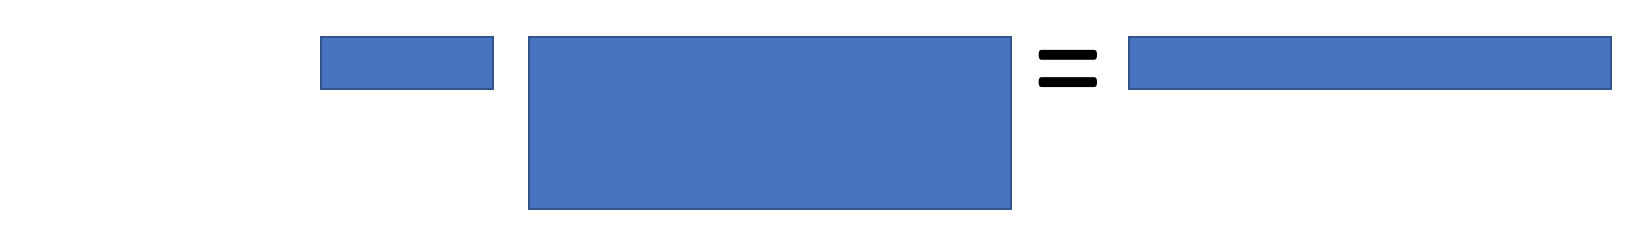
\includegraphics[width=.9\textwidth]{elmSmall}\\
		 \invisible<beamer|1>{\rotatebox{90}{transformed}} & 
		\invisible<beamer|1>{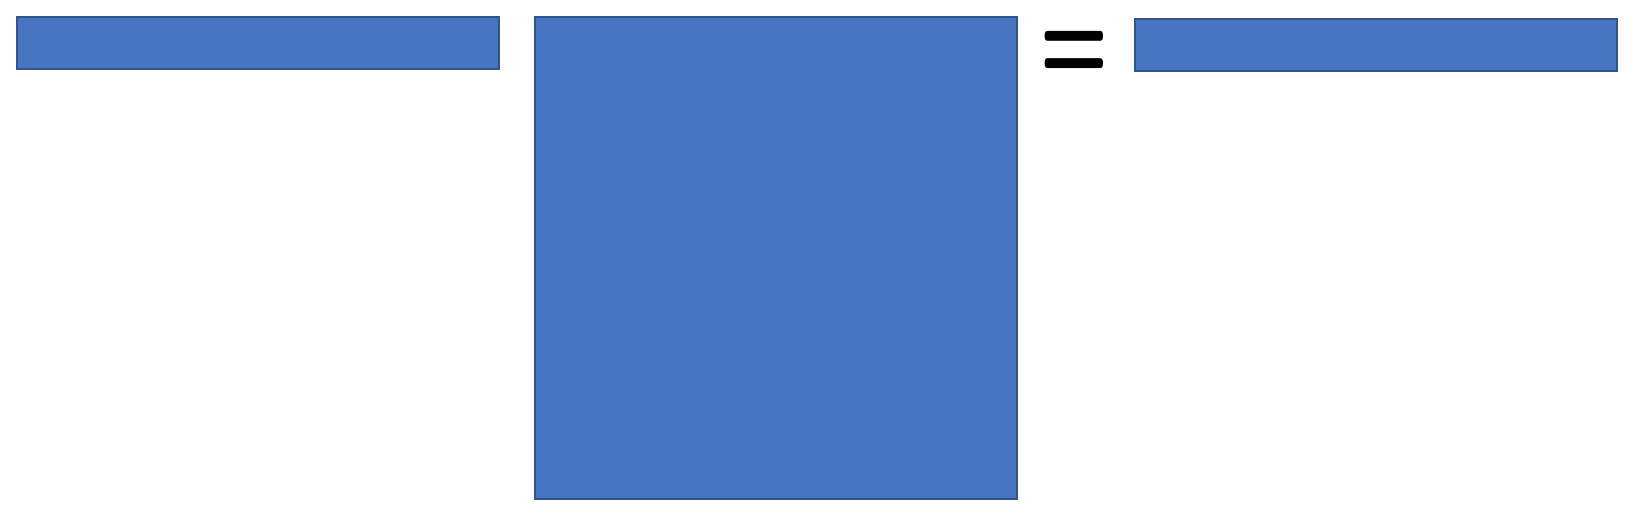
\includegraphics[width=.9\textwidth]{elmBig}}\\
	\end{tabular}
\end{center}

\bigskip

\invisible<beamer|1>{
Remarks
\begin{itemize}
	\item instead of $\bfW \bfY = \bfC$ solve $\hat{\bfW} \sigma(\bfK \bfY)  = \bfC$
	\item solve bigger problem $\leadsto$ memory, computation, \ldots
	\item what happens to ${\rm rank}(\sigma(\bfK\bfY))$ when $\sigma(x)=x$?
\end{itemize}}

\only<beamer|2>{}
\end{frame}




\begin{frame}[fragile]\frametitle{Conjecture: Universal Approximation Properties}

Given the data $\bfY \in \R^{n_f \times n}$ and $\bfC \in \R^{n_c \times n}$
with $n\gg n_f$, there is nonlinear function $\sigma:\R \to \R$, a matrix $\bfK \in \R^{m \times n_f}$, and a bias $\bfb \in \R^m$ such that

$$
 {\rm rank}(\sigma(\bfK \bfY + \bfb)) = n.
$$

\bigskip
\pause
Therefore, possible~\cite{Cybenko1989,HornikEtAl1989} to find ${\bfW}\in\R^{n_c\times m}$

$$\bfW \sigma( \bfK \bfY + \bfb) = \bfC.$$

\end{frame}


\begin{frame}[fragile]\frametitle{Choosing Nonlinear Model}

$$ \bfW  \sigma(\bfK \bfY+ \bfb)= \bfC $$
\begin{itemize}
\item how to choose $\sigma$?
\pause
\begin{itemize}
	\item early days: motivated by neurons
	\item popular choice: $\sigma(x) = \tanh(x)$ (smooth, bounded, \ldots)
	\item nowadays: $\sigma(x) = \max(x,0)$ (aka ReLU, rectified linear unit, non-differentiable, not bounded, simple)
\end{itemize}
\pause
\item how to choose $\bfK$ and $\bfb$?
\pause
\begin{itemize}
	\item pick randomly $\leadsto$ branded as \emph{extreme learning machines}~\cite{HuangEtAl2006}
	\item train (optimize) $\leadsto$ done for most neural network
	\item \emph{deep learning} when neural network has many layers
\end{itemize}
\end{itemize}


\end{frame}

\begin{frame}\frametitle{First Experiment: Random Transformation}

Select activation function and choose $\bfK$ and $\bfb$ randomly and solve the least-squares/classification problem

\bigskip

The Pros:
\begin{itemize}
\item universal approximation theorem: can interpolate any function
\item very(!) easy to program
\item can serve as a benchmark to more sophisticated methods
\end{itemize}

\bigskip

Some concerns:
\begin{itemize}
\item may require very large $\bfK$ (scale with $n$, number of examples)
\item may not generalize well
\item large dense linear algebra
\end{itemize}

\begin{center}
	\texttt{EELM\_Peaks.m}
\end{center}
\end{frame}


\begin{frame}[allowframebreaks]
	\frametitle{References}
\bibliographystyle{abbrv}
\bibliography{NumDNN}
\end{frame}

\end{document}




